% document formatting
\documentclass[10pt]{article}
\usepackage[utf8]{inputenc}
\usepackage[left=1in,right=1in,top=1in,bottom=1in]{geometry}
\usepackage[T1]{fontenc}
\usepackage{xcolor}

% math symbols, etc.
\usepackage{amsmath, amsfonts, amssymb, amsthm}

% lists
\usepackage{enumerate}

% images
\usepackage{graphicx} % for images
\usepackage{tikz}

% code blocks
\usepackage{minted, listings} 

% verbatim greek
\usepackage{alphabeta}

\newcommand{\dd}{\text{d}}

\graphicspath{{./assets/images/Week 7}}

\title{02-712 Week 7 \\ \large{Biological Modeling and Simulation}}
 
\author{Aidan Jan}

\date{\today}

\begin{document}
\maketitle

\section*{Non-Linear Models (Deterministic)}

\subsection*{SIR Models}
Susceptible, Infected, Recovered model.
\begin{itemize}
	\item These models are particularly useful for epidemiology.  We can write $S$, $I$, and $R$ as differential equations in terms of time:
	\begin{align*}
        S(t) &= \dots\\
        I(t) &= \dots\\
        R(t) &= \dots
    \end{align*}
\end{itemize}
For the purposes of an example, suppose that once recovered, infected people become susceptible again.
\begin{center}
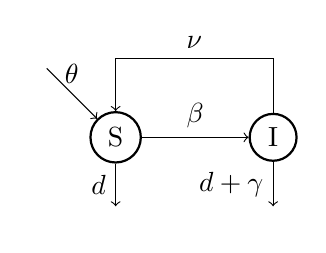
\begin{tikzpicture}
    \node[thick, circle, draw] at (1, 1) (S) {S};
    \node[thick, circle, draw] at (3, 1) (I) {I};
    \node at (1, 0) (deadS) {};
    \node at (3, 0) (deadI) {};
    \node at (0, 2) (preS) {};
    \node at (1, 2) (toS) {};

    \draw[->] (S) edge node[above] {$\beta$} (I);
    \draw[->] (preS) edge node[above] {$\theta$} (S);
    \draw[->] (S) edge node[left] {$d$} (deadS);
    \draw[->] (I) edge node[left] {$d + \gamma$} (deadI);
    \draw (I) -- (3, 2) -- node[above] {$\nu$}(1, 2) -- (1, 1.8);
    \draw[->] (toS) edge (S);
\end{tikzpicture}
\end{center}

From this drawing, we can write the differential equations:
\begin{align*}
    \frac{\dd S}{\dd t} &= \theta + vI - dS - \beta SI\\
    \frac{\dd I}{\dd t} &= \beta SI - I(\nu + (\gamma + d))
\end{align*}
In this case, because of the $\beta SI$ term, we have a nonlinear model.  (That term is degree 2 in terms of the two variables, $d$ and $I$.)

\subsubsection*{Solving Differential Equations}
For a model like this, we want to find the equilibrium.  Therefore, we can set both the derivatives to 0, since that denotes a balanced system.  We get:
\begin{align*}
    0 &= \theta - ds - \nu I - \beta SI \\
    0 &= \beta SI - I(\nu + (\gamma + d))
\end{align*}
Now, we can begin to simplify:
\begin{align*}
    \begin{cases}
        0 &= \theta - ds^* - \beta S^* I^* + \nu I^*\\
        0 &= \beta S^* I^* - (d + \nu + \gamma) I^*
    \end{cases}\\
    \begin{cases}
        0 &= \theta - ds^* - \beta S^* I^* + \nu I^*\\
        0 &= \beta I^* (S^* - (d + \nu + \gamma))
    \end{cases}
\end{align*}
The possible solutions are either:
\begin{align*}
    \begin{cases}
        I^* &= 0 \\
        S^* &= \frac{\theta}{d}
    \end{cases}\\
    \begin{cases}
        S^* &= \frac{d + \gamma + \nu}{\beta}\\
        I^* &= \frac{\theta - \frac{d}{\beta} (d + \gamma + \nu)}{d + \nu}
    \end{cases}
\end{align*}
The first case implies that disease is absent.  The second implies we have an endemic.

\subsubsection*{Prediction}
Suppose we have the $I^* = 0$ starting case.  Let's add a perturbation, $\epsilon_I$.  What happens?
\begin{itemize}
	\item We can plug in $S = S^* + \epsilon_S$ and $I = I^* + \epsilon_I$ into our system to find out!  If the number of $I$ increases to infinity, it represents the disease spreading at a rapid pace.  If nothing happens, it implies that the system is stable.
	\item As it turns out, studying these $\epsilon$ values (perturbations) is easier than studying the system as a whole.  We can actually write the epsilon values in their own differential equations by plugging $S = S^* + \epsilon_S$ and $I = I^* + \epsilon_I$ into the original differential equations:
	\begin{align*}
        \frac{\dd \epsilon_S}{\dd t} &= \frac{\dd}{\dd t} (S - S^*) = \frac{\dd S}{\dd t} = \theta - d(S^* + \epsilon_S) - \beta (S^* + \epsilon_S)(I^* + \epsilon_I) + \nu (I^* + \epsilon_I)\\
        \frac{\dd \epsilon_S}{\dd t} &= \frac{\dd}{\dd t} (I - I^*) = \frac{\dd I}{\dd t} = \beta (S^* + \epsilon_S)(I^* + \epsilon_I) - (d + \nu + \gamma) (I^* + \epsilon_I)
    \end{align*}
    \item Now, because we are studying small numbers, we can assume that the $\epsilon$ values are tiny, e.g., $\epsilon_S, \epsilon_I << 1$ and $\epsilon_S \cdot \epsilon_I = 0$.
    \item With this, we can rewrite our system:
    \begin{align*}
        \frac{\dd \epsilon_S}{\dd t} &= (\theta - dS^* - \beta S^* I^* + \nu I^*) - (d \epsilon_S - \beta S^* \epsilon_I - \beta I^* \epsilon_S + \gamma \epsilon_I)\\
        \frac{\dd \epsilon_I}{\dd t} &= (\beta S^* I^* - dI^* - \nu I^* - \gamma I^*) + (-d\epsilon_I - \nu \epsilon_I - \gamma \epsilon_I + \beta S^* \epsilon_I + \beta I^* \epsilon_S)
    \end{align*}
    \item We can actually simplify this by a lot by dropping the first term.  (We can do this because the first term is the equilibrium equations, which we set to equal zero.)
    \begin{align*}
        \frac{\dd \epsilon_S}{\dd t} &= - (d \epsilon_S - \beta S^* \epsilon_I - \beta I^* \epsilon_S + \gamma \epsilon_I)\\
        \frac{\dd \epsilon_I}{\dd t} &= (-d\epsilon_I - \nu \epsilon_I - \gamma \epsilon_I + \beta S^* \epsilon_I + \beta I^* \epsilon_S)
    \end{align*}
    \item Now, we can write this system in matrix form:
    \[\begin{bmatrix} \frac{\dd \epsilon_S}{\dd t} \\ \frac{\dd \epsilon_I}{\dd t} \end{bmatrix} = M \begin{bmatrix} \epsilon_S \\ \epsilon_I \end{bmatrix}\]
    where
    \[M = \begin{bmatrix} -\beta I^* - d & -\beta S^* + \gamma \\ \beta I^* & \beta S^* - (d + \nu + \gamma) \end{bmatrix}\]
    \item We can study the eigenvectors and eigenvalues.
    \begin{itemize}
        \item If $r_1 = \beta \frac{\theta}{d} - (d + \nu + \gamma) > 1$, then it means that the disease will spread.
    \end{itemize}
\end{itemize}

\section*{Numerical Integration Methods (ODEs)}
Recall normal integration:
\begin{itemize}
	\item "Area under the curve"
	\item Riemann sum breaks the area into tiny rectangles (or $x$-intervals) and sums them
\end{itemize}
Using this technique we can derive the forward euler method

\subsection*{Forward Euler Method}
\[\frac{\dd y}{\dd t} = f(t, y) \rightarrow y(t)\]
Write the derivative as
\[\frac{\dd y}{\dd t} = y' = \lim_{\Delta t = 0}\frac{y(t + \Delta t) - y(t)}{\Delta t}\]
Note that we can write
\[y(t + \Delta t) = y(t) + \Delta t y'(t) = y(t) + f(t, y) \Delta t\]
Alternatively, if we take the timestep approach (e.g., defining functions recursively), we can write
\[y(t_{n + 1}) = y_{n + 1} = y_n + f(t_n, y_n) \Delta t\]
With this, you are able to estimate the value of the next point in time based on the current point and the time step.  You can start from a known point, then "walk along the slope" until you get to your desired $t$-value.
\begin{itemize}
	\item The main pro for this is that it is very easy to implement, and allows you to estimate the next point without having to integrate.
	\item However, the further you go, the more inaccurate it gets.  To minimize this, the step size $\Delta t$ should be minimized.
\end{itemize}

\subsection*{Backward Euler Method}
Suppose we have
\begin{align*}
    \frac{\dd y}{\dd t} &= f(t, y)\\
    y(t_0) &= y_0
\end{align*}
Now, we use the equation similar to the forward Euler method, but instead of adding $\Delta t$, we subtract it:
\[y(t - \Delta t) \sim y(t) - f(t, y) \Delta t\]
From this, we can derive the following, assuming $t \equiv t_{i + 1}$ and $t - \Delta t \equiv t_i$
\[y_{i + 1} = y_i + f(t_{i + 1}, y_{i + 1}) \Delta t + \theta(\Delta t^2)\]
This is an implicit method rather than an explicit method like the forward euler's method.  We need to isolate the $y_{i + 1}$ somehow.  The $\theta(\Delta t^2)$ term is an error term from the taylor series that we can ignore.
\begin{itemize}
	\item Due to this being implicit, it is really only useful if we know the function, because then we can just plug in.  However, if we have to find the function, it is hard to use.  Instead, we can use the midpoint method.
\end{itemize}

\subsection*{Midpoint Method}
Similar to Taylor methods from earlier.  We start with 
\begin{align*}
    y(t_i + \Delta t) &= y_{i + 1}\\
    y(t_i - \Delta t) &= y_{i - 1}
\end{align*}
We can expand both to degree 3 in taylor expansion.
\begin{align*}
    y_{i + 1} &= y_i + \Delta t f(t_i, y_i) + \frac{\Delta t^2}{2} f'(t_i, y_i) + \theta(\Delta t^3)\\
    y_{t - 1} &= y_i - \Delta t f(t_i, y_i) + \frac{\Delta t^2}{2} f'(t_i, y_i) + \theta(\Delta t^3)
\end{align*}
Now, we can subtract them, and the square and cubed terms cancel out.
\[y_{i + 1} - y_{i - 1} = 2\Delta t f(t_i, y_i)\]
From here, we can rearrange to solve for $y_{i + 1}$.
\[y_{i + 1} = y_{i - 1} + 2 \Delta t f(t_i, y_i)\]
\begin{itemize}
	\item Intuitively, what this basically does is suppose you are at $t_1$ and you want to get to $t_2$.  The earlier formula tries to estimate the value at $t_2$ using the point $t_1$ and the slope at $t_1$.  
	\item Instead, what this method does is it estimates $t_2$ using the current point at $t_1$, but the slope at the midpoint between $t_1$ and $t_2$.  Therefore, it is more accurate compared to before.
\end{itemize}



\end{document}